

\renewcommand{\EntradaBibtex}{MarcoNuno_Revista_2018_03_00}
%\setcounter{footnote}{0}

\begin{frame}{\citetitle{\EntradaBibtex} \footnotemark[1]}
\begin{columns}
\begin{column}{0.4\textwidth}
		Componentes:
		\begin{itemize}
		\item Un teléfono inteligente y una pulsera inteligente que extrae los datos de signos vitales del paciente
		\item Una aplicación WEB donde el médico o un familiar a cargo del paciente puede obtener estadísticas de interés.
		\end{itemize}
\end{column}
\begin{column}{0.6\textwidth}  
    \begin{center}
     %%%%% this is a minipage, so \textwidth is already adjusted to the size of the column
     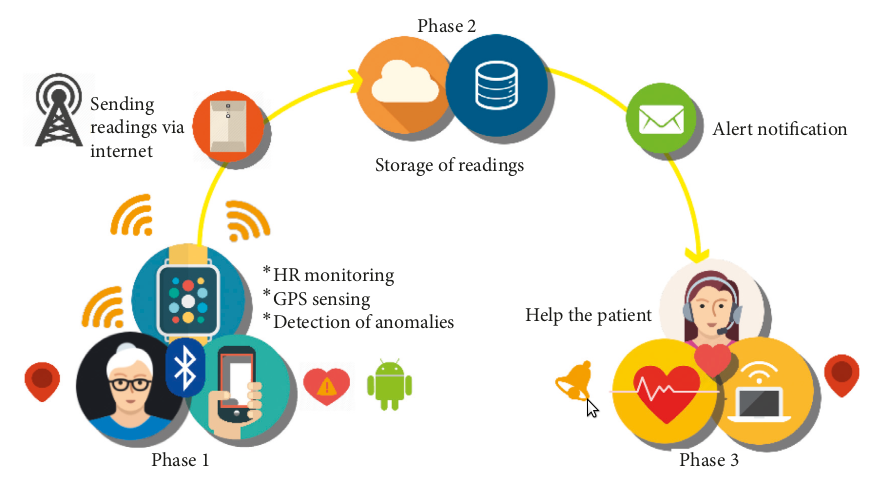
\includegraphics[width=0.8\textwidth]{Figs/SignosVitales1}
     \end{center}
\end{column}
\end{columns}
\footnotetext[1]{\fullcite{\EntradaBibtex}}
\end{frame}

\begin{frame}{\citetitle{\EntradaBibtex} (2)}

\begin{columns}
\begin{column}{0.5\textwidth}
		Datos extraidos del sistema WEB:
		\begin{itemize}
		\item Historial de ubicación del paciente
		\item Gráficas de evolución de signos vitales (específicamente presión aterial y niveles de estrés)
		\item Manejo de múltiples pacientes
		\end{itemize}
\begin{center}
     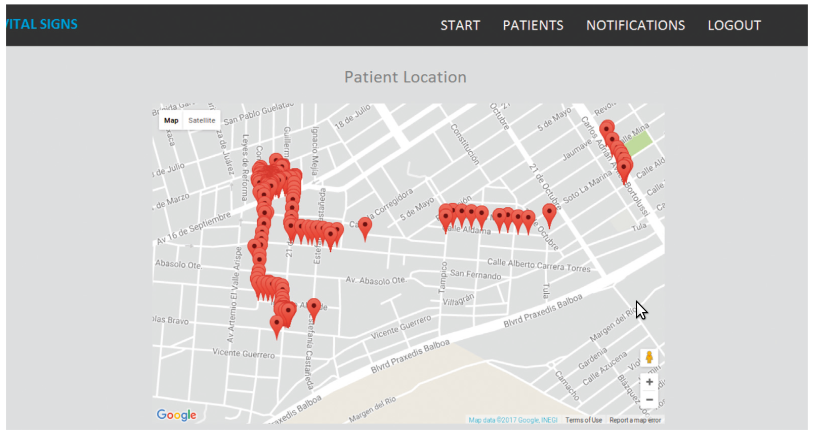
\includegraphics[width=0.8\textwidth]{Figs/SignosVitales4}
     
     \end{center}
\end{column}
\begin{column}{0.5\textwidth}  
    \begin{center}
     %%%%% this is a minipage, so \textwidth is already adjusted to the size of the column
     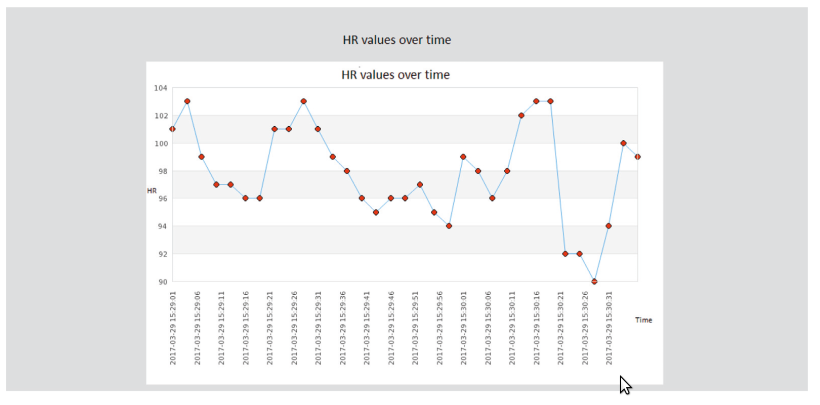
\includegraphics[width=0.8\textwidth]{Figs/SignosVitales2}
	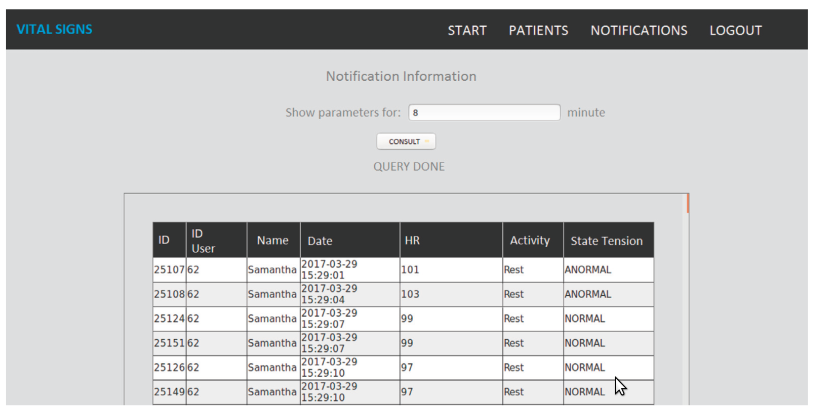
\includegraphics[width=0.8\textwidth]{Figs/SignosVitales3}

     \end{center}
\end{column}
\end{columns}
\end{frame}


